%%%%%%%%%%%%%%%%%%%%%%%%%%%%%%%%%%%%%%%%%%%%%%%%%%%%%%%%
%%%%%%%%%%%%%%%%%%%%%%%%%%%%%%%%%%%%%%%%%%%%%%%%%%%%%%%%
\section{General Concepts}
\label{ml:general}

%%%%%%%%%%%%%%%%%%%%%%%%%%%%%%%%%%%%%%%%%%%%%%%%%%%%%%%%
\subsection{Evaluating Performance}
\label{ml:general:eval}

\subsubsection{Confusion Marix}
\label{ml:general:eval:cm}

The confusion matrix is a simple table of the number of actual, or truth, class instances
versus the number of a model's predicted class instances.
A two class example is provided in \cref{table:CM}.
Multi-class confusion matrices are straight forward extensions,
with correctly classified instances appearing along the diagonal.

\begin{table}[H]
  \centering
  \begin{tabular}{c | c | c | c |}
  \multicolumn{2}{c}{} & \multicolumn{2}{c}{\textbf{Actual}} \\ \cline{3-4}
  \multicolumn{1}{c}{} & & Positive & Negative \\ \cline{2-4}
  \multirow{4}{*}{\rotatebox{90}{\textbf{Predicted}}} & \multirow{2}{*}{Positive} & \multirow{2}{*}{TP} & FP \\[-8pt]
   & & & (Type I) \\ \cline{2-4}
   & \multirow{2}{*}{Negative} & FN & \multirow{2}{*}{TN} \\[-8pt]
   & & (Type II) & \\ \cline{2-4}
  \end{tabular}
  \caption{Two class confusion matrix.}
  \label{table:CM}
\end{table}

\subsubsection{TPR \& TNR -- Sensitivity \& Specificity}
\label{ml:general:eval:TPR_TNR}
The true positive rate (TPR) and true negative rate (TNR) are
relatively straight forward to compute and understand, along with their complements,
the false negative rate (FNR) and false positive rate (FPR).

\begin{enumerate}[noitemsep]
\item True positive rate (TPR), \ie sensitivity, recall, hit rate.
\begin{equation} \label{eq:TPR}
\text{TPR} = \frac{\text{TP}}{\text{P}} = \frac{\text{TP}}{\text{TP}+\text{FN}} = 1 - \text{FNR} = P\left(\hat{+} \mid + \right)
\end{equation}

\item True negative rate (TNR), \ie specificity, selectivity.
\begin{equation} \label{eq:TNR}
\text{TNR} = \frac{\text{NP}}{\text{N}} = \frac{\text{TN}}{\text{TN}+\text{FP}} = 1 - \text{FPR} = P\left(\hat{-} \mid - \right)
\end{equation}
\end{enumerate}

% TODO precision vs recall

% TODO cite in text
\begin{figure}
\centering
  \begin{subfigure}[c]{0.48\textwidth}\centering
  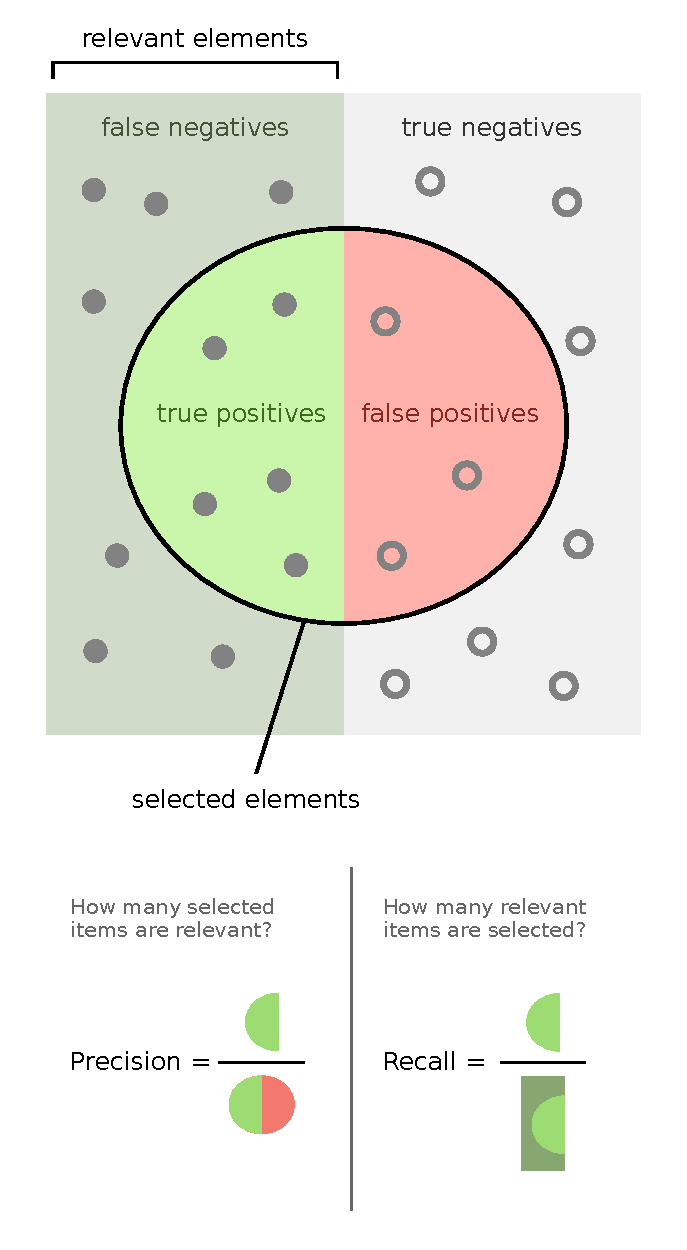
\includegraphics[width=\textwidth]{figures/ml/precision_recall.pdf}
  \caption{Precision \& Recall}
  \label{fig:graphical_CM_quantities:precision_recall}
  \end{subfigure}
  ~
  \begin{subfigure}[c]{0.48\textwidth}\centering
  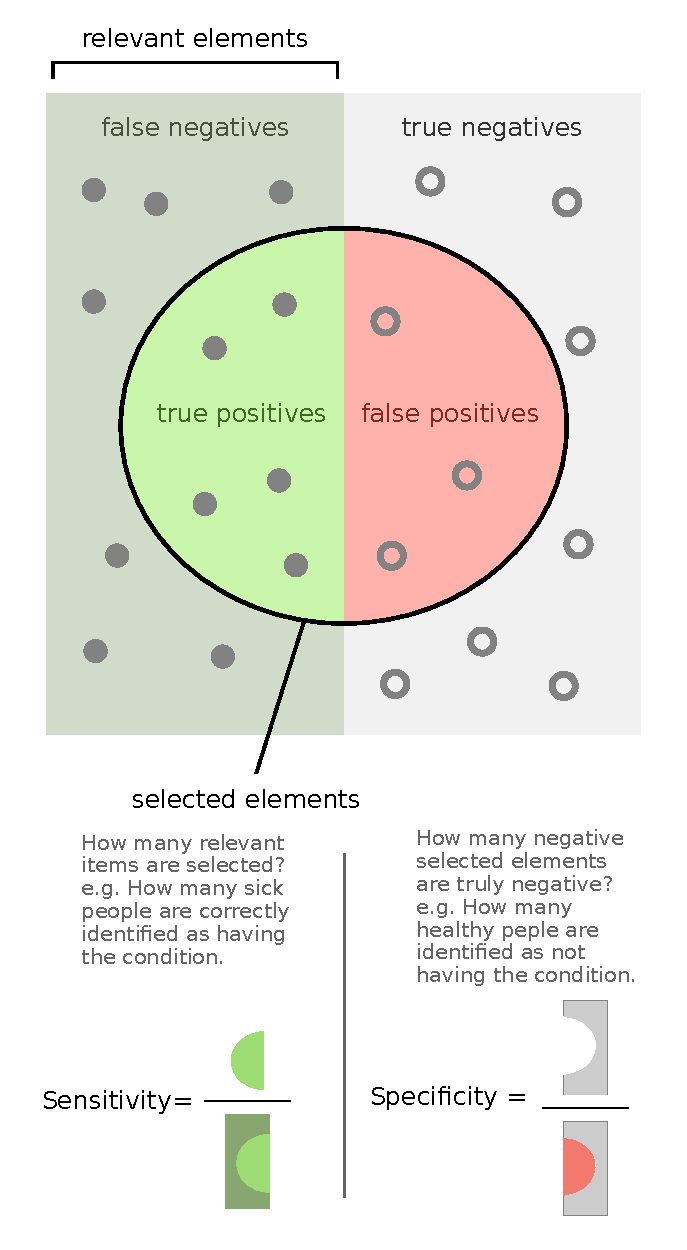
\includegraphics[width=\textwidth]{figures/ml/sensitivity_and_specificity.pdf}
  \caption{Sensitivity \& Specificity}
  \label{fig:graphical_CM_quantities:sensitivity_specificity}
  \end{subfigure}
\caption{
Graphical representation of
precision versus recall, by \href{https://commons.wikimedia.org/wiki/File:Precisionrecall.svg}{Walber},
and
sensitivity versus specificity, by \href{http://en.wikipedia.org/wiki/File:Sensitivity_and_specificity.svg}{FeanDoe}.
}
\label{fig:graphical_CM_quantities}
\end{figure}

% TODO other scores: F1, etc

\subsubsection{ROC Curves}
\label{ml:general:eval:ROC}
% TODO include small figure with TPR vs FPR (better in the upper left), and version with better in lower right

\subsubsection{Selecting a Decision Threshold}
\label{ml:general:eval:decision_threshold}

% include \cref to significance section, if eventually added

In physics we may try to maximize the significance $Z$ of a classifier\footnote{And or
work with the \href{https://en.wikipedia.org/wiki/Neyman\%E2\%80\%93Pearson\_lemma}{Neyman-Pearson framework}.} by
picking an optimal point along the ROC curve to set the decision threshold.
However in data science it is often better to create a payoff matrix of the anticipated
benefits associated with a TP or TN, and costs associated with a FP or FN,
for the particular business case at hand.
The expected value of any decision threshold can quickly be computed
from the payoff matrix elements, $E\left( \hat{A} \mid B\right)$, as

\begin{equation} \label{eq:E_profit}
E\left(\text{profit}\right) = \sum_{A,B} E\left( \hat{A} \mid B\right) P\left(\hat{A} \mid B \right) P\left(B\right),
\end{equation}

\noindent where $A$ and $B$ are any two cases.
The optimal decision threshold can then be found by maximizing $E\left(\text{profit}\right)$.

%%%%%%%%%%%%%%%%%%%%%%%%%%%%%%%%%%%%%%%%%%%%%%%%%%%%%%%%
\subsection{Bias-Variance Tradeoff}
\label{ml:general:biasVar}
% TODO add graphs too

\begin{enumerate}[noitemsep]
\item Bias: Errors due to a model not learning about relationships between features, \ie underfitting.
\item Variance: Errors due to an overly complex model failing to generalize beyond the training data, \ie overfitting.
\end{enumerate}

%%%%%%%%%%%%%%%%%%%%%%%%%%%%%%%%%%%%%%%%%%%%%%%%%%%%%%%%
\subsection{Gradient Decent}
\label{ml:general:gradDec}
% TODO

%%%%%%%%%%%%%%%%%%%%%%%%%%%%%%%%%%%%%%%%%%%%%%%%%%%%%%%%
\subsection{Normalization}
\label{ml:general:normalization}
% TODO normalization of input features (for faster training, more equal regularization), batch renormalization in neural networks

%%%%%%%%%%%%%%%%%%%%%%%%%%%%%%%%%%%%%%%%%%%%%%%%%%%%%%%%
\subsection{Loss Functions}
\label{ml:general:loss_Func}
% TODO log loss, OLS

%%%%%%%%%%%%%%%%%%%%%%%%%%%%%%%%%%%%%%%%%%%%%%%%%%%%%%%%
\subsection{Regularization}
\label{ml:general:reg}
% TODO

\begin{subequations} \label{eq:L1_L2}
\begin{align}
\Omega_{\text{L1}}\left(\bm{\beta}\right) &= \lambda \norm{\bm{\beta}}\,,     \label{eq:L1} \\
\Omega_{\text{L2}}\left(\bm{\beta}\right) &= \lambda \norm{\bm{\beta}}^{2}\,. \label{eq:L2}
\end{align}
\end{subequations}

\subsubsection{L1 -- Lasso}
\label{ml:general:reg:L1}
% TODO taxi cab distance, many model parameters are reduced to 0 (sparsity) - built in feature selection, not as affected by outliers since it is not squared

\subsubsection{L2 -- Ridge}
\label{ml:general:reg:L2}
% TODO computationally fast
% particularly useful when variance of data is high(?)

\subsubsection{Elastic Net}
\label{ml:general:reg:EN}

\begin{equation} \label{eq:elastic_net}
\Omega_{\text{EN}}\left(\bm{\beta}\right) = \lambda_{1} \norm{\bm{\beta}} + \lambda_{2} \norm{\bm{\beta}}^{2}
\end{equation}

% TODO connections to SVM, use cases
